\chapter{نصب \lr{texlive}}\label{chp:chap1}
\thispagestyle{empty}
% \rhead{\leftmark}
\section{دانلود آخرین نسخه}\label{seq1-1}
ابتدا باید ایمیج برنامه را از یکی از میرور‌های سایت CTAN دانلود کنید. دانشگاه یزد در آدرس \\
\url{http://tug.ctan.org/systems/texlive/Images/ }\\
فایل \lr{iso} مربوط به \lr{texlive} را به  اشتراک می گذارد. این فایل iso را باید در ویندوز با یکی از برنامه‌های اجرا گر اصطلاحاً مانت کنیم. در نسخه‌های جدید ویندوز(ویندوز هشت به بعد) با دو بار کلیک روی فایل ایزو خود به خود مانت می‌شود.  در ویندوز‌های قدیمی برای بارگذاری فایل ایمیج می توان از برنامه‌هایی نظیر \lr{poweriso} استفاده کرد. همچنین می توان این ایمیج را روی یک \lr{DVD} رایت نمود و از آن استفاده کرد. برنامه‌های رایت مانند \lr{nero} می‌توانند فایل ایمیج را روی \lr{DVD} بنویسند.
\subsection{نصب روی ویندوز}
دو روند کلی برای نصب
\lr{TeXLive} در این صفحه آموزش داده می‌شود. هر دو روند نتیجه یکسانی را در برخواهند داشت. در هر دو روند فرض شده است که شما 
\lr{DVD}
نصب \lr{TexLive} را به نحوی در اختیار دارید. شکل زیر نمایی از فایل‌های موجود در این \lr{DVD} را برای \lr{TexLive2015} نشان می‌دهد. 
\begin{figure}[h!]
\centering{ 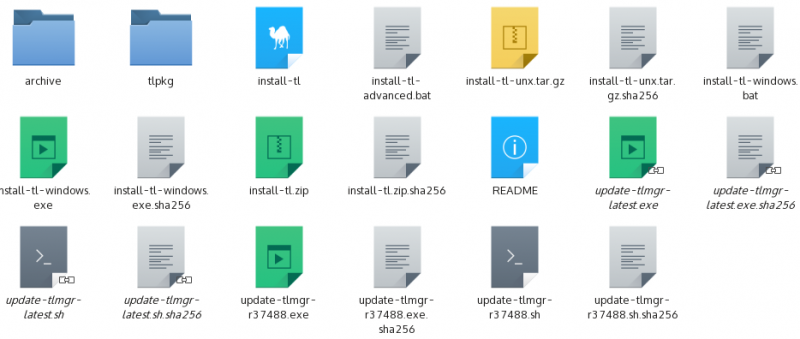
\includegraphics[width=0.65\linewidth]{Texlivefolder}
 \caption{نمایی از فایل ها و فولدرهای موجود در پوشه  \lr{TeXLive2015}}}
\end{figure}
برای مثال فرض کنید که می‌خواهیم \lr{TeXLive2015} را بر روی سیستم‌عامل ویندوز نصب کنیم. ددر روش نصب ساده شما کافی است که پنج گام زیر را طی کنید. البته قبل از آن یقیین حاصل کنید که در درایوی که می‌خواهید 
\lr{TeXLive} را نصب کنید فضای کافی وجود دارد. به عنوان نمونه برای 
\lr{TeXLive2015}
شما نیازمند حدود ۴ تا ۵ گیگ فضا هستید.
\begin{enumerate}
 \item 
 ابتدا اگر توزیع
 \lr{TeX} دیگری دارید، و یا نسخه قدیمی‌تری از 
 \lr{TeXLive}
 را دارید به طور کامل پاک کنید. گرچه نسخه‌های دیگر
 \lr{TeX} و حتی نسخه‌های گذشته 
 \lr{TeXLive} نیز می‌تواند به همراه نسخه جدید وجود داشته باشد، اما بهتر است که این‌کار انجام شود. به عنوان مثال برای پاک کردن نسخه قدیمی 
 \lr{TeXLive} به منوی \lr{Control Panel} بروید و از آن‌جا به بخش \lr{Programs and Features} بروید و \lr{TeXLive} نسخه قدیمی را پاک کنید. 
\begin{figure}[h!]
 \centering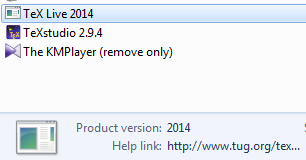
\includegraphics[scale=0.5]{UninstallTexLive}
\end{figure}
با این کار یک صفحه سیاه رنگ باز می‌شود، منتظر بمانید تا پیام \lr{Press any key} ظاهر شود، آن‌گاه می‌توانید یقین کنید که نسخه قبلی \lr{TeXLive} به صورت موفقیت آمیز پاک شده است. 
\begin{figure}[h!]
 \centering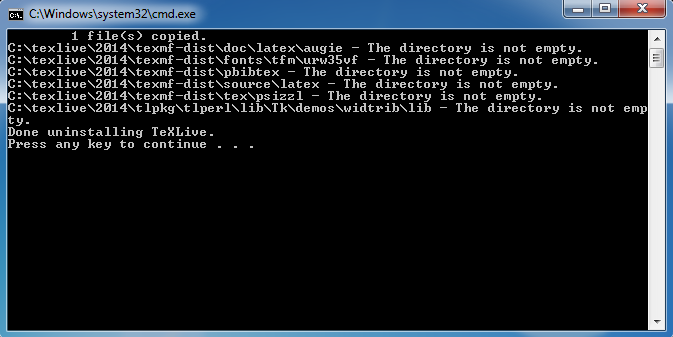
\includegraphics[scale=0.5]{Texliveuninstallcmd}
 \caption{پیام انتهایی در پایان \lr{Uninstall} برنامه \lr{TeXLive}}
\end{figure}
در ضمن می‌توانید باقیمانده فایل‌ها را نیز با مراجعه به پوشه نصب 
\lr{TeXLive} که به صورت پیش‌فرض در پوشه‌ای به نام \lr{texlive} در درایو \lr{C} قرار دارد، پاک کنید. 
\item
به پوشهٔ 
\lr{TeXLive}
بروید. روی فایل \lr{install-tl-advanced.bat} دابل کلیک کنید. (نکته: در ویندوزهای \lr{vista} به بعد باید روی فایل فوق کلیک راست کنید و \lr{Run As Administrator}
را بزنید.) 
\begin{figure}[h!]
 \centering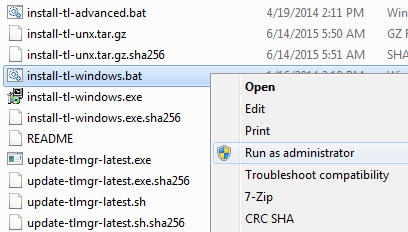
\includegraphics[scale=0.5]{InstallTexLiveRunasAdmin}
 \caption{برای نصب \lr{TeXLive} حتما گزینه \lr{Run as Administrator} را انتخاب کنید.}
\end{figure}
\item
روی \lr{Install TexLive} کلیک کنید تا نصب شروع شود. دقت کنید که در \lr{TeXLive2015} باید چندین پنجره را 
\lr{Next} بزنید تا در آخرین صفحه این دکمه را مشاهده کنید.
\begin{figure}[h!]
 \centering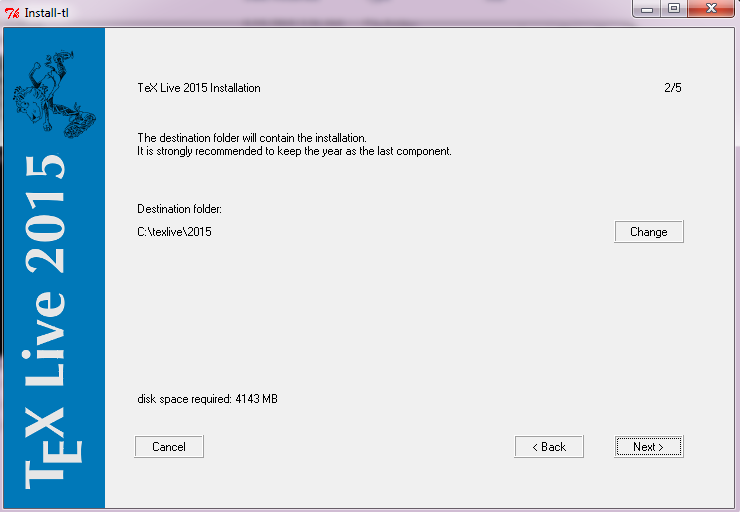
\includegraphics[scale=0.5]{InstallTexLivewindows}
 \caption{در بین صفحات نصب \lr{TeXLive2015} در یک صفحه از شما مسیری که می‌خواهید این برنامه در آن نصب شود، پرسیده می‌شود.}
\end{figure}
\item
بعد از فشردن کلید \lr{Install TexLive} پنچره‌ای به شما نشان داده می‌شود که بیانگر روند نصب بسته‌های \lr{TexLive} است. دقت کنید که به صورت همزمان یک پنجره \lr{cmd} نیز باز است که این پنجره نیز روند نصب را به شما نشان می‌دهد. صبر کنید تا هنگامی که در انتهای نصب باید پیغام \lr{Wellcome to TeX Live} را بگیرید. 
\begin{figure}[h!]
 \centering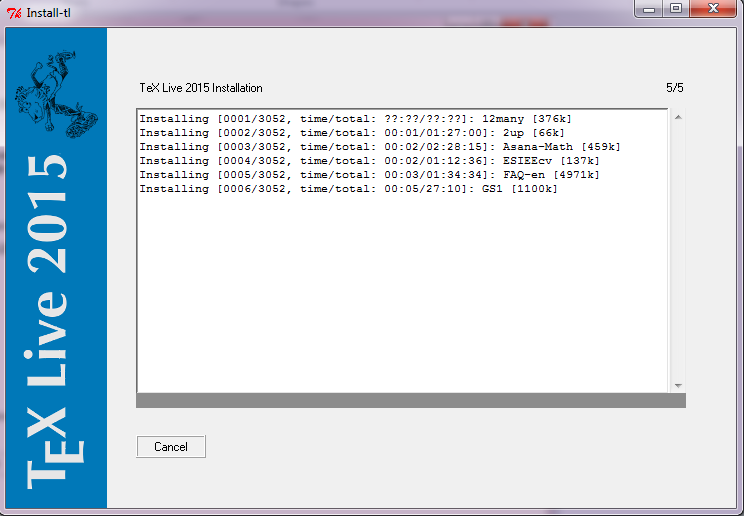
\includegraphics[scale=0.5]{InstallTexLivePackage}
 \caption{پنجره‌ای که در آن روند نصب بسته‌های \lr{LaTeX} نشان داده می‌شود.}
\end{figure}
\item
روی دکمه \lr{Finish} کلیک کنید. 
\end{enumerate}
\subsection{نصب در لینوکس}
دقت کنید که ما در این مجال دستورات را برای لینوکس \lr{Ubuntu} و \lr{Mint} آورده‌ایم. برای مابقی \lr{Linux} ها دقیقا کارهای مشابهی را باید انجام داد. 
\subsubsection{نصب به صورت \lr{command Line}}
ابتدا اگر بسته‌های تک‌لایو از قبل نصب دارید، با زدن دستور زیر در ترمینال حذف کنید.
\begin{latin}
\begin{lstlisting}[style=Mybash]‫
sudo apt-get remove texlive-*
\end{lstlisting}
\end{latin}

یک ترمینال باز کنید. به مسیر پوشه \lr{TeX Live} بروید. لیست فایل‌های موجود در پوشهٔ 
\lr{TeX Live} تقریباً باید به این صورت باشد:
\begin{latin}
\begin{lstlisting}[style=Mybash]
iran@iran:~$ cd /media
iran@iran:/media$ dir
floppy   floppy0  texlive
iran@iran:/media$ cd texlive
iran@iran:/media/texlive$ dir
archive               README
install-tl            rsync
install-tl-advanced.bat       install-tl.bat            tlpkg
install-tl-unx.tar.gz         update-tlmgr-r23180.exe
install-tl-unx.tar.gz.sha256  update-tlmgr-r23180.exe.sha256
install-tl.zip            update-tlmgr-r23180.sh
install-tl.zip.sha256         update-tlmgr-r23180.sh.sha256
\end{lstlisting}
\end{latin}
همانطور که می‌بینید فایلی با نام \lr{install-tl} هست. برای اجرای آن، دستور زیر را بزنید.
\begin{latin}
\begin{lstlisting}[style=Mybash]
sudo perl install-tl
\end{lstlisting}
\end{latin}
پیغام زیر را می‌گیرید.
\begin{latin}
\begin{lstlisting}[style=Mybash]
[sudo] password for iran:
\end{lstlisting}
\end{latin}
چون بصورت \lr{sudo} هست، پسورد کاربر جاری را از شما می‌خواهد. وارد کنید و دکمه \lr{Enter} را بزنید.

پیغام منوهای زیر ظاهر می‌شود.
\begin{latin}
\begin{lstlisting}[style=Mybash]
<O> options:‬
‪   [ ] use letter size instead of A4 by default‬
‪   [X] allow execution of restricted list of programs via \write18‬
‪   [X] create all format files‬
‪   [X] install macro/font doc tree‬
‪   [X] install macro/font source tree‬
‪   [X] after install, use tlnet on CTAN for package updates
 
‪ <V> set up for portable installation‬
 
‪Actions:‬
‪ <I> start installation to hard disk‬
‪ <H> help‬
‪ <Q> quit‬
 
‪Enter command:
\end{lstlisting}
\end{latin}
حرف
\lr{O} (اُ لاتین) را بزنید تا وارد قسمت 
\lr{Options} شوید.

حرف
\lr{L} را بزنید تا 
\lr{symlink}ها ایجاد شوند.

با این کار 
\lr{symlink}ها ایجاد می‌شوند و نیازی به اضافه کردن‌شان به 
\lr{path} سیستم نیست.

۳ تا اینتر بزنید تا مسیرهایی که پیشنهاد می‌دهد تأیید شوند. می‌توانید تغییر دهید، ولی پیشنهاد نمی‌شود.

حرف
\lr{Y} را بزنید تا بارگیری به‌روزرسانی‌های بسته‌ها بعد اتمام نصب انجام نشود. (به‌دلیل ایجاد مشکل احتمالی پیشنهاد نمی‌شود. مگر اینکه سرعت اینترنت عالی داشته باشید. پیشنهاد می‌شود بعد اتمام نصب، این کار را خودتان به جای استفاده از این گزینه، انجام دهید. یا بهتر از آن، مخزن تک‌لایو را بروزرسانی کنید و از روی آن نصب کنید.)حرف\lr{R} را بزنید که به منوی اصلی برگردید.حرف\lr{I}(آی لاتین) را زدم که نصب شروع بشه.بعد از اتمام نصب، این پیغام زیر را داد:
\begin{latin}
\begin{lstlisting}[style=Mybash]
Most importantly, add /usr/local/texlive/2011/bin/i386-linux
 to your PATH for current and future sessions.
 
 Welcome to TeX Live!
Logfile: /usr/local/texlive/2011/install-tl.log
iran@iran:/media/texlive$
\end{lstlisting}
\end{latin}
همان‌طور که می‌بینید، خطایی در مورد نصب نداده است و پیغام 
\lr{Wellcome to TeX Live} داده است.
\subsection{نصب در مکینتاش}
برای نصب تک‌لایو در مکینتاش، در
\lr{Terminal} بزنید:
\begin{latin}
\begin{lstlisting}[style=Mybash]
sudo ./install-tl.bat
\end{lstlisting}
\end{latin}
قبل شروع فرآیند نصب،
\lr{symlink} ها را در قسمت 
\lr{options} فعال کنید. یعنی بعد زدن دستور بالا، و قبل هر کاری دیگر، در پنجرهٔ ترمینال به‌ترتیب بزنید:\\
ابتدا \lr{O} سپس \lr{Y} و در آخر\lr{R} 
\section{نصب ویرایشگر}
شما می‌توانید فایل 
\lr{LaTeX} خود را در هر ویرایشگری به مانند یک 
\lr{Notepad} ساده بنویسید، و سپس با بازکردن یک 
\lr{cmd}
در ویندوز و یا
\lr{Terminal} در لینوکس، کامپایلر مورد نظر را بر روی فایل خود اجرا کنید. به عنوان مثال فایلی به نام 
\lr{sample.tex}
با محتوای زیر را در نظر بگیرید.
\begin{latin}
\begin{lstlisting}[style=Tex]
\documentclass{report}
\usepackage{xepersian}
\settextfont{XB Niloofar}
 \begin{document}
%*\rl{سلام}*)
\end{document}
\end{lstlisting}
\end{latin}
برای کامپایل این فایل کافی است که یک 
\lr{cmd}
یا
\lr{Terminal} در مسیر این فایل باز کنید و کامپایلر 
\lr{XeLaTeX} در آن تایپ کنید.
\begin{latin}
\begin{lstlisting}[style=Mybash]
xelatex sample.tex
\end{lstlisting}
\end{latin}
البته در اکثر ویرایشگرهای
\lr{LaTeX}
به مانند \lr{TeXStudio، TeXMaker} و ... امکاناتی تعبیه شده است که در همان ویرایشگر می‌توانید کامپایل مورد نظر را انجام دهید. پیش‌فرض کامپایل برخی از این ویرایشگرها \lr{pdfLaTeX} است. مسأله‌ای که وجود دارد این است که برای استفاده از بسته \lr{XePersian} می‌بایست کامپایل \lr{XeLaTeX} بر روی فایل خود انجام دهید. در این نوشتار می‌خواهیم این موضوع را مطرح کنیم که چگونه تنظیم پیش‌فرض کامپایلر این ویرایشگر‌ها را تغییر دهیم.
\subsubsection{ویرایشگر \lr{TeXStudio}}
از منوی \lr{option}، گزینه \lr{Configure TexStudio} را انتخاب کنید. از پنجره‌ای که برای شما باز می‌شود، قسمت \lr{Build} را برگزینید. در قسمت \lr{Build} از گزینه \lr{Default Compiler} کامپایلر مورد نظر خود را انتخاب کنید.
\begin{figure}[h!]
 \centering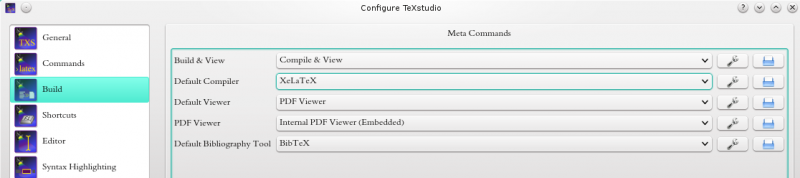
\includegraphics[scale=0.4]{Texstudioxelatex.png}
\end{figure}
البته دقت کنید که با این کار شما کامپایلر پیش‌فرض را کلا تغییر می‌دهید. اما ممکن است که شما فقط بخواهید کامپایلر پیش‌فرض بر روی \lr{XeLaTeX} باشد، اما اکنون بنا به دلیلی بخواهید دوباره \lr{pdflatex} کامپایل کنید، نیازی نیست کامپایلر پیش‌فرض را دوباره تغییر دهید. برای این‌کار از منوی \lr{Tools} قسمت \lr{Command} می‌توانید کامپایلر دلخواه خود را انتخاب کنید.
\begin{figure}[h!]
 \centering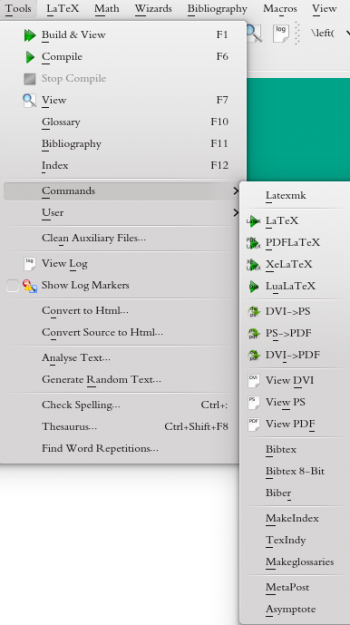
\includegraphics[scale=0.3]{Texstduianothercopmiler.png}
 \end{figure}
\subsubsection{ ویراشگر \lr{TeXmaker}}
در ویرایشگر \lr{TeXmaker} نیز از منوی \lr{option} گزینه \lr{Configure TeXmaker} را انتخاب کنید. به قسمت \lr{Quick Build} بروید. در آن‌جا می‌توانید کامپایلر مورد نظر خود را انتخاب کنید.
\begin{figure}[h!]
 \centering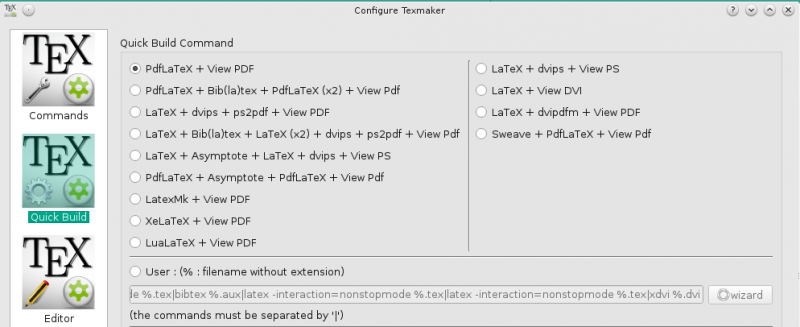
\includegraphics[width=0.80\linewidth]{TexmakerQuickbuild.png}
 \end{figure}
البته دقت کنید که با این کار شما تنظیم \lr{Quick Build} را عوض می‌کنید. در صفحه اصلی این ویرایشگر شما علاوه بر انتخاب \lr{Quick Build} می‌توانید کامپایلر مورد نظر خود را به صورت دستی نیز انتخاب کنید.
\begin{figure}[h!]
 \centering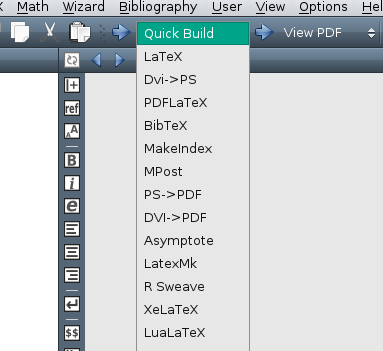
\includegraphics[scale=0.7]{Texmakermanual.png}
 \end{figure}
 
در هر ادیتوری می‌توان کدهای لاتک را نوشت اما ادیتور‌هایی هستند که به صورت گرافیکی نوشتن در محیط لاتک را آسان می‌کنند. یکی از بهترین این ادیتورها 
\lr{kile} است که می توانید از 
\href{https://kile.sourceforge.io/download.php}{https://kile.sourceforge.io/download.php}
نسخه مطلوب را برای سیستم عامل ویندوز  و یا کد منبع آن را برای سیستم عامل لینوکس دانلود کنید. همچنین با استفاده از دستور زیر در لینوکس‌ ابونتو یا مینت می‌توانید آن را نصب نمایید. تنظیمات در ان ادیتور‌ها نیز مشابه بالاست.
\begin{latin}
\begin{lstlisting}[style=Mybash]
sudo apt-get update
sudo apt-get install kile
\end{lstlisting}
\end{latin}
ادیتور‌های زیادی هستند که از لاتک برای نوشتن پشتیبانی می‌کنند منتهی برای زبان فارسی شاید مشکلاتی ایجاد کنند.
بعد از نصب \LR{TeXLive} و ادیتور می‌توانید نوشتن را شروع کنید.
\section{ساختار فایل‌های لاتک}
هر فایل لاتک از سه بخش اصلی تشکیل می‌شود. 
\begin{latin}
\begin{lstlisting}[style=Tex]
%document type
\documentclass[11pt,twoside,a4paper]{article}
%preiamble
\usepackage{xepersian}
\settextfont{XB Niloofar}
%main text
 \begin{document}
%*\rl{سلام}*)
\end{document}
\end{lstlisting}
\end{latin}
 بخش اول نوع سند را مشخص می‌کند. نوع سند می‌تواند مقاله،کتاب ، نامه و یا گزارش باشد(\lr{article, report, book, letter}). که این کلاسها به صورت پیشفرض در لاتک قرار دارند که همراه با آن نصب می شوند. برخی کلاسهای دیگر پیشفرض نیز در زیر آمده است. کلاسهای مختلفی را می‌توان در اینترنت پیدا کرد. کلاس این پایان‌نامه که iut-thesis.cls است را در پوشه آن می توانید بیابید.
   \begin{table}[h]
    \begin{latin}
  \begin{center}
 \begin{tabular}{|m{0.2\linewidth}|m{0.75\linewidth}|}
 \hline
article & For articles in scientific journals, presentations, short reports, program documentation, invitations, ...\\\hline
IEEEtran & For articles with the IEEE Transactions format.\\\hline
proc & A class for proceedings based on the article class.\\\hline
report & For longer reports containing several chapters, small books, thesis, ...\\\hline
book & For real books.\\\hline
slides & For slides. The class uses big sans serif letters.\\\hline
memoir & For changing sensibly the output of the document. It is based on the book class, but you can create any kind of document with it \\\hline
letter & For writing letters.\\\hline
beamer & For writing presentations (see LaTeX/Presentations).\\\hline
  \end{tabular}
    \end{center}
 \end{latin}
  \caption{جدول برخی کلاسهای در لاتک}
 \end{table}
 
 در همین قسمت می توان اندازه فونت پیشفرض، اندازه کاغذ و برخی ماهیت‌های سند را نیز تنظیم نمود. این ماهیت‌ها از قرار زیراند.
   \begin{table}[h!]
    \begin{latin}
  \begin{center}
 \begin{tabular}{|m{0.2\linewidth}|m{0.75\linewidth}|}
 \hline
 10pt, 11pt, 12pt &Sets the size of the main font in the document. If no option is specified, 10pt is assumed. \\\hline
a4paper, letterpaper,...&Defines the paper size. The default size is letterpaper; However, many European distributions of TeX now come pre-set for A4, not Letter, and this is also true of all distributions of pdfLaTeX. Besides that, a5paper, b5paper, executivepaper, and legalpaper can be specified. \\\hline
fleqn &Typesets displayed formulas left-aligned instead of centered. \\\hline
leqno &Places the numbering of formulas on the left hand side instead of the right. \\\hline
titlepage, notitlepage&Specifies whether a new page should be started after the document title or not. The article class does not start a new page by default, while report and book do.\\\hline
twocolumn &Instructs LaTeX to typeset the document in two columns instead of one.\\\hline
twoside, oneside&Specifies whether double or single sided output should be generated. The classes article and report are single sided and the book class is double sided by default. Note that this option concerns the style of the document only. The option twoside does not tell the printer you use that it should actually make a two-sided printout.\\\hline
landscape &Changes the layout of the document to print in landscape mode.\\\hline
openright, openany &Makes chapters begin either only on right hand pages or on the next page available. This does not work with the article class, as it does not know about chapters. The report class by default starts chapters on the next page available and the book class starts them on right hand pages.\\\hline
draft &makes LaTeX indicate hyphenation and justification problems with a small square in the right-hand margin of the problem line so they can be located quickly by a human. It also suppresses the inclusion of images and shows only a frame where they would normally occur.
\\\hline
  \end{tabular}
    \end{center}
 \end{latin}
  \caption{جدول برخی تنظیمات کلاسهای در لاتک}
 \end{table}
 
 بخش دوَم \lr{preiamble} است که محل واردکردن بسته‌های مختلف لاتک برای منظور های مختلف است. همچنین تنظیمات دیگر مربوط به بسته‌ها و یا تعریف متغییرها در این قسمت وارد می شود. از آنجایی که ما از بسته xepersian برای نوشتن فارسی استفاده می‌کنیم این بسته باید آخرین بسته‌ای باشد که فراخوانی می‌شود. هر بسته‌ای برای خود و چگونگی استفاده از آن روی اینترنت مستندات مربوط به خود را دارد.
 
 بخش سوَم مربوط به نوشتار متن و ساختار آن است. در این بخش ما از دستورات مختلف لاتک برای نوشتن سندی که می خواهیم به دست آوریم استفاده می کنیم. از فرامینی که بسته‌های لاتک در اختیار ما قرار می دهند بهره می گیریم تا به وسیله آنها فرمولها، تصاویر،زیرنویس‌ها، جداول، فصول، مراجع و... را بنویسیم. در فصل آینده دستوراتی را که در این بخش استفاده می کنیم و همچنین بسته‌های مرتبط با آنها را معرفی می‌نماییم.
